\chapter{Backend}
Damit die Nutzer der App interaktiv miteinander kommunizieren können, ist eine Verbindung zu einem Server (im weiteren als Backend bezeichnet) nötig.
Daten wie Klassenräume und Nachrichten können unter Angabe von validen Anmeldedaten abgefragt werden.
Als Schnittstelle zwischen der App und dem Backend findet eine REST-API Verwendung.
Die Datenbank verwaltet alle Daten wie Klassenräume, eingestellte Nachrichten und Anmeldedaten.
Eine Grundsätzliche Struktur der Architektur der Komposition von SQL-Datenbank, REST-API und App ist in Abbildung \ref{pic:backendArchitektur} dargestellt.
\begin{figure}[H]
	\begin{center}
	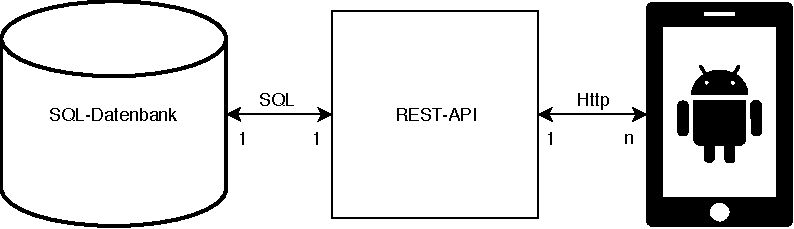
\includegraphics[scale=0.8]{Resources/BackendArchitektur}
	\caption{Architektur des Backends}
	\label{pic:backendArchitektur}
	\end{center}
\end{figure}

\section{Datenbank}
Zur Verwaltung der Anmeldedaten, Klassenräume, Nachrichten und Abonnements wird eine relationale Datenbank eingesetzt.
Die Tabelle \enquote{Persons} enthält die Anmeldedaten (E-Mailadresse und Passwort) jedes Nutzers, sowie dessen jeweilige Rolle (Student, Dozent, Admin).
In \enquote{Messages} sind die Nachrichten gespeichert, die Dozenten in ihre Kursräume einstellen. Jede Nachricht ist einem Kursraum eindeutig zugeordnet und erhält eine eindeutige id. Im Feld \enquote{Payload} ist der eigentliche Text der Nachricht abgespeichert.
Kursraum werden in der Tabelle \enquote{Classrooms} verwaltet.
Jedem Raum ist ein Dozent eindeutig zugeordnet.
Über die \enquote{subscribes} wird die n:m-Beziehung zwischen Studenten und Kursräumen modelliert; sie enthält die Abonnements aller Studenten.
Abbildung \ref{pic:entityRelationship} zeigt detailliert die Struktur der Datenbank.
\begin{figure}[H]
	\begin{center}
	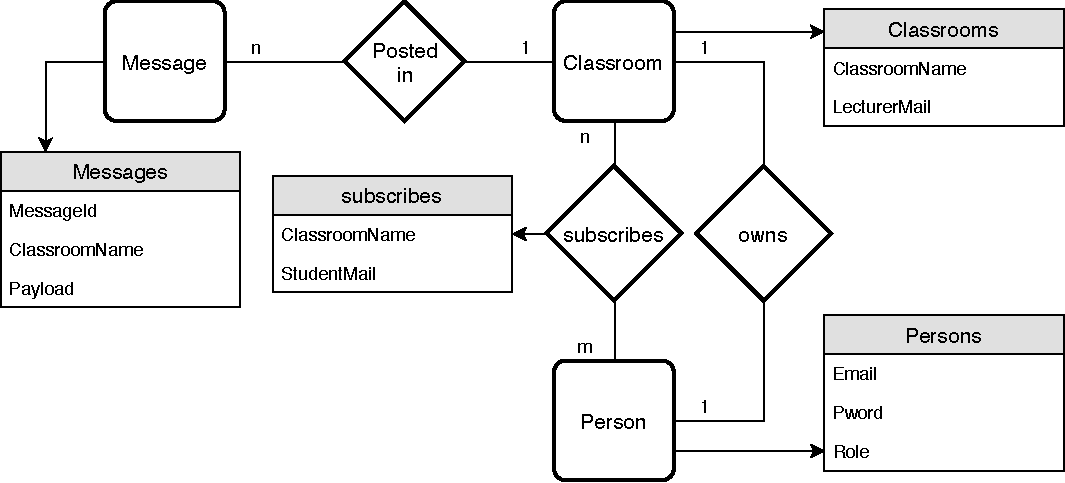
\includegraphics[scale=0.8]{Resources/EntityRelationship}
	\caption{Entity-Relationship Modell der Datenbank}
	\label{pic:entityRelationship}
	\end{center}
\end{figure}
\section{REST-API}
Als Schnittstelle zwischen Backend und App dient eine RESTful-API.
Verschiedene Daten sind über Endpoints (siehe Tabelle \ref{table:endpoints}) abrufbar, welche jeweils mit einer eindeutigen URI adressiert sind. 
Jeder dieser Endpoints ist einem bestimmtem Anwendungsfall zugeordnet, zum Abrufen der Daten muss der Http-Client einen POST-Request senden, der die geforderten Argumente im JSON-Format enthält.
Für Besseres Verständnis ist in Abbildung \ref{pic:rest} ein Beispiel angegeben: für den Login sendet die App einen POST-Request, welcher die Anmeldedaten enthält; der Server antwortet dann mit der Rolle des zugehörigen Benutzers.
Der Vorteil dieser Art von Schnittstelle liegt darin, dass das Backend \textit{stateless} -- also ohne Wissen über den Status des Clients -- implementiert werden kann.
Jedoch müssen bei der Abfrage jeder Ressource die Anmeldedaten des Benutzers gesendet werden.
Darüber hinaus gestaltet sich so die Umsetzung der Serverstruktur als einfach, da sie so ohne Nebeneffekt erweiterbar ist.
Der Hauptgrund für die Wahl einer RESTful-Schnittstelle ist jedoch, dass sie unabhänig vom System implementiert werden kann. 
Es wäre also beispielsweise ohne weiteres möglich neben der App auch eine Webanwendung zu erstellen, welche sich ebenfalls mit dem Backend verbindet.

\begin{figure}[H]
	\begin{center}
	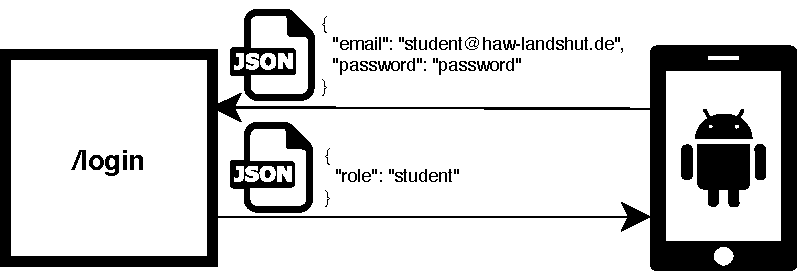
\includegraphics[scale=0.8]{Resources/RESTAPI}
	\caption{Beispiel für Kommunikation mit der REST-API}
	\label{pic:rest}
	\end{center}
\end{figure}

\begin{table}[H]
\begin{tabular}{l|l|l}
\textbf{Endpoint URI} & \textbf{Argumente}  & \textbf{Rückgabewert}\\ \cline{1-3}
/classrooms/all & Student-Anmeldedaten & alle Kursräume und Status  \\ \cline{1-3}
/classrooms/subscribed & Student-Anmeldedaten & alle abonnierten Kursräume \\ \cline{1-3}
/classrooms/subscribe & Student-Anmeldedaten, Kursraumname & Erfolg \\ \cline{1-3}
/classrooms/unscribe & Student-Anmeldedaten, Kursraumname & Erfolg \\ \cline{1-3}
/classrooms/create & Dozent-Anmeldedaten, Kursraumname & Erfolg \\ \cline{1-3}
/classrooms/delete & Dozent-Anmeldedaten, Kursraumname & Erfolg \\ \cline{1-3}
/classrooms/owned & Dozent-Anmeldedaten & alle Dozenten-Kursraume\\ \cline{1-3}
/login & Anmeldedaten & Benutzerrolle \\ \cline{1-3}
/messages/student & Student-Anmeldedaten & abonnierte Nachrichten \\ \cline{1-3}
/messages/create & Dozent-Anmeldedaten, Kursraumname, Text &  Erfolg\\ \cline{1-3}
/messages/delete & Dozent-Anmeldedaten, id & Erfolg\\ \cline{1-3}
/messages/classroom & Anmeldedaten, Kursraumname & Kursraumnachrichten\\ \cline{1-3}
\end{tabular}
\caption{Liste aller Endpoints und deren Argumente beziehungsweise Rückgabewerte}
\label{table:endpoints}
\end{table}